%%%%%%%%%%%%%%%%%%%% veg_white.tex %%%%%%%%%%%%%%%%%%%%%%%%%%%%%
%
% sample root file for the chapters of your "monograph"
%
% Use this file as a template for your own input.
%
%%%%%%%%%%%%%%%% Springer-Verlag %%%%%%%%%%%%%%%%%%%%%%%%%%


% RECOMMENDED %%%%%%%%%%%%%%%%%%%%%%%%%%%%%%%%%%%%%%%%%%%%%%%%%%%
% Fixes vector warnings
\let\accentvec\vec
    \documentclass[graybox,envcountchap,sectrefs]{svmono}
    \let\spvec\vec
    \let\vec\accentvec
\usepackage{amsmath}

\usepackage{mathptmx}
\usepackage{helvet}
\usepackage{courier}

%
\usepackage{type1cm}

\usepackage{makeidx}         % allows index generation
\usepackage{wrapfig}
\usepackage{graphicx}        % standard LaTeX graphics tool
                             % when including figure files
\graphicspath{{Figures/}}
\usepackage{multicol}        % used for the two-column index
\usepackage[bottom]{footmisc}% places footnotes at page bottom

%%% The following removes the Springer label from the book
\usepackage{xpatch}
\makeatletter
\xpatchcmd{\@maketitle}{{\Large Springer\par}}{}{}{}
\makeatother

% see the list of further useful packages
% in the Reference Guide

\makeindex             % used for the subject index
                       % please use the style svind.ist with
                       % your makeindex program

%%%%%%%%%%%%%%%%%%%%%%%%%%%%%%%%%%%%%%%%%%%%%%%%%%%%%%%%%%%%%%%%%%%%%
% Header Description

\usepackage{newtxtext,newtxmath} % <--- not mathptmx
\usepackage{fancyhdr}

\pagestyle{fancy}
\fancyhf{}
\fancyhead[RE]{\runheadsize\runheadstyle\leftmark}
\fancyhead[LO]{\runheadsize\runheadstyle\rightmark}
\fancyhead[LE,RO]{\runheadsize\runheadstyle\thepage}
\fancypagestyle{plain}{%
  \renewcommand{\headrulewidth}{0pt}%
  \fancyhf{}%
  \fancyfoot[RE,LO]{\runheadsize\runheadstyle\thepage}%
}
\makeatletter
\renewcommand\chaptermark[1]{%
  \markboth{%
    \if@chapnum\thechapter\thechapterend\hskip\betweenumberspace\fi #1%
  }{%
    \if@chapnum\thechapter\thechapterend\hskip\betweenumberspace\fi #1%
  }%
}
\renewcommand{\sectionmark}[1]{%
  \markright{%
    \ifnum\c@secnumdepth>\z@ \thesection\seccounterend\hskip\betweenumberspace\fi #1%
  }%
}
\makeatother

\begin{document}

\title{Creating Vegvisir: A Partition Tolerant Blockchain}
\subtitle{A White Paper}
\author{Danny Adams, Gloire Rubambiza, Xinwen Wang, and Robbert van Renesse}
\frontmatter%%%%%%%%%%%%%%%%%%%%%%%%%%%%%%%%%%%%%%%%%%%%%%%%%%%%%%
\let\cleardoublepage\clearpage
\maketitle
\tableofcontents

%%%%%%%%%%%%%%%%%%%%%%acronym.tex%%%%%%%%%%%%%%%%%%%%%%%%%%%%%%%%%%%%%%%%%
% sample list of acronyms
%
% Use this file as a template for your own input.
%
%%%%%%%%%%%%%%%%%%%%%%%% Springer %%%%%%%%%%%%%%%%%%%%%%%%%%

\extrachap{Acronyms}

We have included a list of commonly used acronyms that are common in this white
paper. The document does explain the context in which these terms are applied;
however, the reader will has the responsibility to investigate terms a deeper
understanding is desired.

Lists of abbreviations\index{acronyms, list of},
symbols\index{symbols, list of} and the like are easily formatted with the help
of the Springer-enhanced \verb|description| environment.

\begin{description}
\item[CRDT]{Conflict-free Replicated Data Types}
\item[DAG]{Directed Acyclic Graph}
\end{description}


\extrachap{Introduction}

As presented in its introductory paper\cite{karlsson2018vegvisir}, Vegvisir is
a tamperproof log that is often defined as a blockchain. It differs from other
implementations in the fact it is low powered and does not require a
stable network connectivity. In this paper, we will define 3 fundamental parts
of the Vegvir structure:
\begin{enumerate}
    \item Vegvisir Core
    \item Hardware Interface
    \item Application Interface
\end{enumerate}

The \emph{Core} references the autonomous agent responsible for managing the
tamperproof log and the subsequent CRDT list. The \emph{Hardware Interface}
concerns the aspect of information transfer over a connection. This interface
is utilized by the agent to gather or send information concerning the data
structure. The \emph{Application Interface} is utilized to interact with the
log.

\mainmatter%%%%%%%%%%%%%%%%%%%%%%%%%%%%%%%%%%%%%%%%%%%%%%%%%%%%%%%

\chapter{General Abstractions}
% Abstractis a description of the chapter that would be available online.
% Description will not appear in print.
\abstract*{General Abstractions is the overview of all the state machine. The
mechanisms describe are required for the Vegvisir structure to be enabled to
work as described in the original paper. It is possible to have additional
methods or functions within an agent.}

\section{The State Machine}
\label{sec:1}
A state machine can be generally described as an autonomous agent that is
encoded with variables to define its state. The machine transitions to
different states by when given commands. In Vegvisir, the state machine is
responsible for managing two items:
\begin{enumerate}
    \item Blockdag
    \item CRDT List
\end{enumerate}


\section{Blockdag}
The blockdag, or a DAG of \emph{blocks}, is the key structure for the protocol.
The state variables of Vegvisir are the blocks that are defined in the next
section. In this section, we will describe the blocks, their orientation in the
framework, the Block cache, and the reconcilliation protocol. 

\subsection{Block}
A \textbf{block} is a public key certificate that consists of:
\begin{itemize}
    \item a \emph{header}
    \begin{itemize}
        \item{identifier of the creator of the block}
        \item{list of hashes of the parent blocks}
    \end{itemize}
    \item a \emph{body}
        \begin{itemize}
            \item{list of \emph{transactions}}
                \begin{itemize}
                    A \emph{transaction} is a pair. (\textbf{topic, event}
                    \footnote{events are CRDTs. Additional information in
                     \ref{pubsub}})
                \end{itemize}
        \end{itemize}
    \item signature of the creator
        \begin{itemize}
            \item{The signed items include the header and body}
        \end{itemize}
\end{itemize}
A block is uniquely identified within a structure by the hash over all of its
contents. Within the structure, there exists one unique block that has no
parent hashes. The name of this block is the \textbf{genesis block}.

\subsection{Blockdag}
The blockdag structure can be defined as a DAG where the vertices are
the blocks. The edges are originating at vertex and point towards the vertex
described by the vertex's parent hash. The structure has the following
constraints:
\begin{enumerate}
    \item{There exists a unique genesis block AND it is the \emph{sole} sink vertex}
    \item{There exists a path from every block to the genesis block}
    \item{There exists \textbf{no} edge $b_1 \rightarrow b_2$ if there is 
    another path $b_1$ to $b_2$}
\end{enumerate}
The \textbf{frontier set} is the set of blocks on the DAG that have no
successors (sources, given that blocks in the DAG point to their parent
blocks).


\section{CRDT List}


\chapter{Vegvisir Core}
% Abstractis a description of the chapter that would be available online.
% Description will not appear in print.
\abstract*{This chapter is dedicated to the creation of the Vegsir Core.
Definitions of key components, data structure defined, and the description of
the basic operations that are performed within the core.}

\section{The State Machine}
\label{sec:1}
A state machine can be generally described as an autonomous agent that is
encoded with variables to define its state. The machine transitions to
different states by when given commands. In Vegvisir, the state machine is
responsible for managing the following items:
\begin{enumerate}
    \item Blockdag
    \item Block cache
    \item CRDT List
\end{enumerate}


\section{Blockdag}
The blockdag, or a DAG of \emph{blocks}, is the key structure for the protocol.
The state variables of Vegvisir are the blocks that are defined in the next
section. In this section, we will describe the blocks, their orientation in the
framework, the Block cache, and the reconcilliation protocol. 

\subsection{Block}
A \textbf{block} is a public key certificate that consists of:
\begin{itemize}
    \item a \emph{header}
    \begin{itemize}
        \item{identifier of the creator of the block}
        \item{list of hashes of the parent blocks}
    \end{itemize}
    \item a \emph{body}
        \begin{itemize}
            \item{list of \emph{transactions}}
                \begin{itemize}
                    A \emph{transaction} is a pair. (\textbf{topic, event}
                    \footnote{events are CRDTs. Additional information in
                     \ref{pubsub}})
                \end{itemize}
        \end{itemize}
    \item signature of the creator
        \begin{itemize}
            \item{The signed items include the header and body}
        \end{itemize}
\end{itemize}
A block is uniquely identified within a structure by the hash over all of its
contents. Within the structure, there exists one unique block that has no
parent hashes. The name of this block is the \textbf{genesis block}.

\subsection{Blockdag}
The blockdag structure can be defined as a DAG where the vertices are
the blocks. The edges are originating at vertex and point towards the vertex
described by the vertex's parent hash. The structure has the following
constraints:
\begin{enumerate}
    \item{There exists a unique genesis block AND it is the \emph{sole} sink vertex}
    \item{There exists a path from every block to the genesis block}
    \item{There exists \textbf{no} edge $b_1 \rightarrow b_2$ if there is 
    another path $b_1$ to $b_2$}
\end{enumerate}
The \textbf{frontier set} is the set of blocks on the DAG that have no
successors (sources, given that blocks in the DAG point to their parent
blocks).


\section{CRDT List}


\chapter{Application Level Interfaces}
% Abstractis a description of the chapter that would be available online.
% Description will not appear in print.
\abstract*{General Abstractions is the overview of all the state machine. The
mechanisms describe are required for the Vegvisir structure to be enabled to
work as described in the original paper. It is possible to have additional
methods or functions within an agent.}
\section{Publish  Subscribe Implementation and API} \label{pubsub}
In addition to the blockdag abstraction, nodes offer a simplified
publish/subscribe abstraction.  There is a list of topics, and a node can
subscribe to topics and publish to topics. The interface/implementation is
something like this:
\begin{itemize}
    \item{ \textbf{prepare}(topic, event): create a new (topic, event)
     transaction without publishing}
    \item{ \textbf{flush}(): add one or more blocks with prepared transactions.
    \\The order of the transactions in the blocks should correspond to the
     order of preparation.}
    \item{ \textbf{subscribe}(topic, listener):  listener(event) is invoked
     each time a new event is received for the given topic.  Events are posted
     in a total order that is consistent with the partial order of the events
     in the blockdag.}
\end{itemize}
We will provide CRDT libraries so that applications can update CRDTs when they
receive events.  Note that each block in a blockdag has a well-defined CRDT
state.


\include{Contents/chapter_4}
%%%%%%%%%%%%%%%%%%%%%%acknow.tex%%%%%%%%%%%%%%%%%%%%%%%%%%%%%%%%%%%%%%%%%

\chapter{Closing Remarks}
\section{Acknowledgements}
The documentation is part of an ongoing group effort of many collaborators. The
work would not have been possible to complete without the work of many
students: ( We should list all of them HERE).  Additionally, this work was
partially funded NSF (CSR-1422544) and NIST (60NANB15D327 and 70NANB17H181),
Cisco, Intel, Facebook, Infosys, and Amazon.

% We have not discussed if or what to be included in an Appendix. Keeping
% The template here prior
%\section*{Appendix}
%\addcontentsline{toc}{section}{Appendix}


% Reference Section
\bibliographystyle{abbrv}
% argument is your BibTeX string definitions and bibliography database(s)
\bibliography{references}
\label{reference}

%%%%%%%%%%%%%%%%%%%%%% appendix.tex %%%%%%%%%%%%%%%%%%%%%%%%%%%%%%%%%
%
% sample appendix
%
% Use this file as a template for your own input.
%
%%%%%%%%%%%%%%%%%%%%%%%% Springer-Verlag %%%%%%%%%%%%%%%%%%%%%%%%%%

\appendix
\motto{All's well that ends well}
\chapter{Chapter Heading}
\label{introA} % Always give a unique label
% use \chaptermark{}
% to alter or adjust the chapter heading in the running head

Use the template \emph{appendix.tex} together with the Springer document class SVMono (monograph-type books) or SVMult (edited books) to style appendix of your book in the Springer layout.


\section{Section Heading}
\label{sec:A1}
% Always give a unique label
% and use \ref{<label>} for cross-references
% and \cite{<label>} for bibliographic references
% use \sectionmark{}
% to alter or adjust the section heading in the running head
Instead of simply listing headings of different levels we recommend to let every heading be followed by at least a short passage of text. Furtheron please use the \LaTeX\ automatism for all your cross-references and citations.


\subsection{Subsection Heading}
\label{sec:A2}
Instead of simply listing headings of different levels we recommend to let every heading be followed by at least a short passage of text. Furtheron please use the \LaTeX\ automatism for all your cross-references and citations as has already been described in Sect.~\ref{sec:A1}.

For multiline equations we recommend to use the \verb|eqnarray| environment.
\begin{eqnarray}
\vec{a}\times\vec{b}=\vec{c} \nonumber\\
\vec{a}\times\vec{b}=\vec{c}
\label{eq:A01}
\end{eqnarray}

\subsubsection{Subsubsection Heading}
Instead of simply listing headings of different levels we recommend to let every heading be followed by at least a short passage of text. Furtheron please use the \LaTeX\ automatism for all your cross-references and citations as has already been described in Sect.~\ref{sec:A2}.

Please note that the first line of text that follows a heading is not indented, whereas the first lines of all subsequent paragraphs are.

% For figures use
%
\begin{figure}[t]
\sidecaption[t]
%\centering
% Use the relevant command for your figure-insertion program
% to insert the figure file.
% For example, with the option graphics use
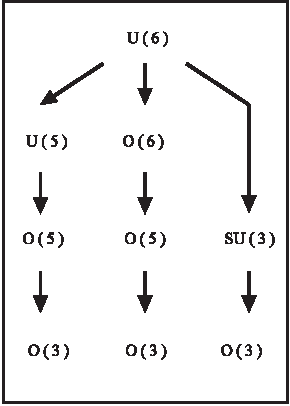
\includegraphics[scale=.65]{figure}
%
% If not, use
%\picplace{5cm}{2cm} % Give the correct figure height and width in cm
%
\caption{Please write your figure caption here}
\label{fig:A1}       % Give a unique label
\end{figure}

% For tables use
%
\begin{table}
\caption{Please write your table caption here}
\label{tab:A1}       % Give a unique label
%
% For LaTeX tables use
%
\begin{tabular}{p{2cm}p{2.4cm}p{2cm}p{4.9cm}}
\hline\noalign{\smallskip}
Classes & Subclass & Length & Action Mechanism  \\
\noalign{\smallskip}\hline\noalign{\smallskip}
Translation & mRNA$^a$  & 22 (19--25) & Translation repression, mRNA cleavage\\
Translation & mRNA cleavage & 21 & mRNA cleavage\\
Translation & mRNA  & 21--22 & mRNA cleavage\\
Translation & mRNA  & 24--26 & Histone and DNA Modification\\
\noalign{\smallskip}\hline\noalign{\smallskip}
\end{tabular}
$^a$ Table foot note (with superscript)
\end{table}
%


\backmatter%%%%%%%%%%%%%%%%%%%%%%%%%%%%%%%%%%%%%%%%%%%%%%%%%%%%%%%
%%%%%%%%%%%%%%%%%%%%%%%acronym.tex%%%%%%%%%%%%%%%%%%%%%%%%%%%%%%%%%%%%%%%%%
% sample list of acronyms
%
% Use this file as a template for your own input.
%
%%%%%%%%%%%%%%%%%%%%%%%% Springer %%%%%%%%%%%%%%%%%%%%%%%%%%

\Extrachap{Glossary}


Use the template \emph{glossary.tex} together with the Springer document class SVMono (monograph-type books) or SVMult (edited books) to style your glossary\index{glossary} in the Springer layout.


\runinhead{glossary term} Write here the description of the glossary term. Write here the description of the glossary term. Write here the description of the glossary term.

\runinhead{glossary term} Write here the description of the glossary term. Write here the description of the glossary term. Write here the description of the glossary term.

\runinhead{glossary term} Write here the description of the glossary term. Write here the description of the glossary term. Write here the description of the glossary term.

\runinhead{glossary term} Write here the description of the glossary term. Write here the description of the glossary term. Write here the description of the glossary term.

\runinhead{glossary term} Write here the description of the glossary term. Write here the description of the glossary term. Write here the description of the glossary term.
%\Extrachap{Solutions}

\section*{Problems of Chapter~\ref{intro}}

\begin{sol}{prob1}
The solution\index{problems}\index{solutions} is revealed here.
\end{sol}


\begin{sol}{prob2}
\textbf{Problem Heading}\\
(a) The solution of first part is revealed here.\\
(b) The solution of second part is revealed here.
\end{sol}


\printindex

%%%%%%%%%%%%%%%%%%%%%%%%%%%%%%%%%%%%%%%%%%%%%%%%%%%%%%%%%%%%%%%%%%%%%%
\end{document}
